\begin{center}
    \section{Validaci\'on del modelo}
\end{center}

\noindent
\justify

Para la validaci\'on del modelo CFD-DEM desarrollado, se aplic\'o el modelo para resolver el problema de Fessler \& Eaton$^{\cite{Fessler1999}}$, en donde se investig\'o el efecto de la turbulencia generada por part\'iculas de cobre de $70 [\mu m]$ de di\'ametro sobre un flujo \textit{orientado hacia atr\'as}, como se muestra en la Figura \ref{problemaVal}.

\begin{figure}[h!]
    \centering
    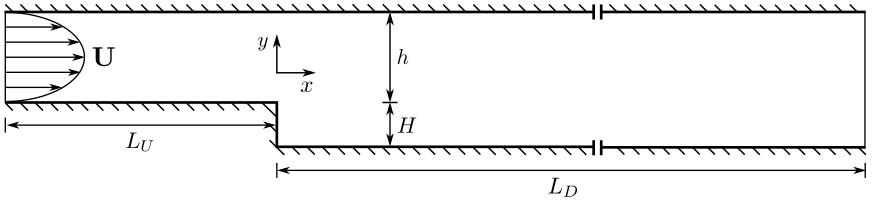
\includegraphics[width=0.75\textwidth]{Images/Fessler.PNG}
    \caption{Geometr\'ia de estudio.}
    \label{problemaVal}
\end{figure}

\subsection{Descripci\'on del problema}

\noindent
\justify

En 1999, Fessler \& Eaton estudiaron el efecto de part\'iculas de vidrio y cobre de distintos tama\~nos ($70$, $90$ y $150 [\mu m]$ de di\'ametro), a diferentes cargas m\'asicas (entre el 3 y el 40 \% del flujo m\'asico) y a las mismas condiciones experimentales de velocidad y presi\'on de flujo en donde se apreci\'o una atenuaci\'on del nivel de turbulencia relacionada con un decaimiento en el n\'umero de Stokes de las part\'iculas.

\noindent
\justify

La motivaci\'on detr\'as de esta investigaci\'on recae en la complejidad de las interacciones entre part\'iculas peque\~nas y densas con la fase turbulenta de una sustancia gaseosa; adem\'as de la importancia en diferentes casos, de car\'acter industrial y natural, en donde se producen flujos particulados que son, muchas veces, inentendidos. En pocos aspectos, tales como la dispersi\'on de part\'iculas en flujos homog\'eneos, se pueden llevar a cabo estudios anal\'iticos con altos niveles de precisi\'on. Sin embargo, la mayor\'ia de los casos en la realidad comprenden flujos heterog\'eneos y anisotr\'opicos sujetos a inestabilidades, con marcadas variaciones entre flujo y flujo, que imposibilitan el desarrollo de un modelo matem\'atico anal\'itico que defina a cabalidad la naturaleza de los flujos y que sea, a su vez, lo suficientemente preciso. 

\noindent
\justify

Se ha reportado en la literatura que los niveles de turbulencia pueden ser moderados con la ayuda de la carga de diferentes masas. Investigaciones como la de Hetsroni$^{\cite{Hetsroni1989}}$ y Gore \& Crowe$^{\cite{Gore1991}}$ establecieron los cimientos del comportamiento turbulento en la interacci\'on fluido - part\'icula; mientras que en investigaciones desarrolladas por Kulick, Fessler \& Eaton$^{\cite{Kulick1994}}$ y Tsuji, Morikawa \& Shiomi$^{\cite{Tsuji1984}}$ se demostr\'o que la atenuaci\'on de la turbulencia incrementa tanto con la carga m\'asica como con el n\'umero de Stokes de las part\'iculas.  

\noindent
\justify

En el presente estudio se investig\'o el comportamiento de las part\'iculas sobre un flujo \textit{orientado hacia atr\'as} (Figura \ref{problemaVal}). Este flujo es ideal para el estudio de la interacci\'on part\'icula-turbulencia debido a que las estad\'isticas del flujo medio son conocidas como \textit{invariables} debido a la presencia de part\'iculas s\'olidas$^{\cite{Kulick1994}}$; hecho esencial que garantiza que los cambios en la turbulencia se deben \'unicamente a la presencia de material particulado, dado que los flujos separados son sensibles al perfil de velocidad media. En este trabajo se emplearon part\'iculas de vidrio de $90$ y $150 [\mu m]$ de di\'ametro y part\'iculas de cobre de $70 [\mu m]$; que proveen dos diferentes part\'iculas con n\'umeros de Stokes distinto y tres diferentes valores de Reynolds. 

\begin{table}[h!]
	\centering
	\begin{tabular}{|c|c|}
		\hline
		\textbf{Par\'ametro} & \textbf{Valor} \\ \hline
		Altura $H$ & $26.7 [mm]$ \\ \hline
		Rango de expansi\'on & 5:3 \\ \hline
		Relaci\'on de aspecto & 17:1 \\ \hline
		Velocidad inicial $U_0$ & $9.39 [m/s]$ \\ \hline
		$Re_H = \frac{U_0 H}{\mu}$ & $18400$ \\ \hline
		$\tau _f$, gran escala de tiempos de remolino, $\frac{5H}{U_0}$ & $12.7 [ms]$ \\ \hline
	\end{tabular}
	\caption{Par\'ametros del flujo.}
	\label{dataFlow}
\end{table}

\noindent
\justify

\subsection{Desarrollo experimental}

\noindent
\justify

El flujo sufre una expansi\'on unidireccional en donde se evita la sedimentaci\'on de part\'iculas. El n\'umero de Reynolds de la entrada fue de $13800$ con una velocidad en la l\'inea central de $10.5 [m/s]$. El rango de expansi\'on fue de $\frac{5}{3}$; mientras que la relaci\'on de aspecto es de 17:1. Hecho que garantiza un flujo bidimensional a trav\'es de una porci\'on importante del experimento.

\noindent
\justify

El condicionamiento del flujo de entrada, el flujo de salida y el sistema de alimentaci\'on de part\'iculas se ilustra en la Figura \ref{experimento}. El sistema provee velocidad de flujo uniforme con carga de part\'iculas en la entrada. Un canal de $5.2 [m]$ asegura el completo desarrollo del flujo y contempla el tiempo suficiente para que las part\'iculas lleguen al equilibrio con el medio circundante. Se emple\'o un ventilador, con frecuencia variable, como sistema de control m\'asico.

\begin{figure}[h!]
	\centering
	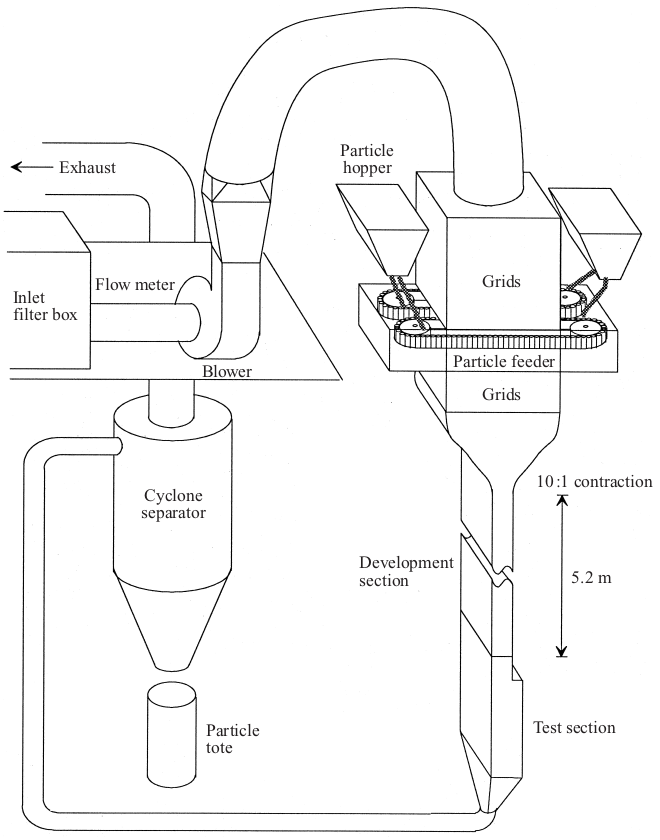
\includegraphics[width=0.7\textwidth]{Images/experimento.png}
	\caption{Esquema del montaje experimental$^{\cite{Fessler1999}}$.}
	\label{experimento}
\end{figure}

\subsubsection{Descripci\'on particular}

\noindent
\justify

El n\'umero de Reynolds que define el movimiento particular est\'a definido por la Ecuaci\'on \ref{Rep}.

\begin{equation}
	Re_p = \frac{d_p U_{rel}}{\mu}
	\label{Rep}
\end{equation}

\noindent
\justify

De la Ecuaci\'on \ref{Rep}: $d_p$ es el di\'ametro de la part\'icula, $\mu$ es la viscosidad cinem\'atica y $U_{rel}$ es la escala de velocidad que caracteriza la velocidad de deslizamiento medio de la part\'icula sobre el flujo.

\noindent
\justify

El n\'umero de Stokes es la relaci\'on entre el tiempo de respuesta de las part\'iculas con respecto a la escala de tiempo representativa en el flujo.

\begin{equation}
	St = \frac{\tau _p}{\tau _f}
	\label{Stp}
\end{equation}

\noindent
\justify

Para part\'iculas peque\~nas con n\'umeros de Reynolds despreciables, Stokes (1851) demostr\'o que la constante de tiempo particular se define con base en la Ecuaci\'on \ref{Stps}.

\begin{equation}
	\tau _{p, Stokes} = \frac{\left(2 \rho _p + \rho _f \right) d_p ^2}{36 \mu}
	\label{Stps}
\end{equation}

\noindent
\justify

El coeficiente de arrastre $C_D$, para n\'umeros de Reynolds superiores a $700$, puede calcularse con base en la Ecuaci\'on \ref{CD_700}.

\begin{equation}
	C_D = \frac{24}{Re_p} \left(1 + 0.15 Re_p ^{0.687} \right)
	\label{CD_700}
\end{equation}

\noindent
\justify

El incremento en el coeficiente de arrastre como el del n\'umero de Reynolds disminuir\'a la constante de tiempo particular; de modo que la constante de tiempo modificada empleada en este estudio se puede apreciar en la Ecuaci\'on \ref{taup}.

\begin{equation}
	\tau _p = \frac{\tau _{p, stokes}}{1 + 0.15 Re_p ^{0.687}}
	\label{taup}
\end{equation}

\noindent
\justify

La escala de tiempo representativa en el flujo se calcul\'o con base en la Ecuaci\'on \ref{tauf}.

\begin{equation}
	\tau _f = \frac{5H}{U_0}
	\label{tauf}
\end{equation}

\subsubsection{M\'etodos experimentales}

\noindent
\justify

Todas las velocidades de flujo fueron medidas a trav\'es de un anem\'ometro l\'aser Doppler (LDA, por sus siglas en ingl\'es). Cada punto de dato representa 2000 muestras individuales de velocidad que mantiene la incertidumbre estad\'istica desde $\pm 0.02 [m/s]$ hasta $\pm 0.08 [m/s]$. Para medir la velocidad de las part\'iculas, se emple\'o una t\'ecnica de discriminaci\'on por amplitud de pedestal, apreciable en la Figura \ref{medicion}. A partir de all\'i, se estim\'o un error experimental cercano al $5\%$. 

\begin{figure}[h!]
	\centering
	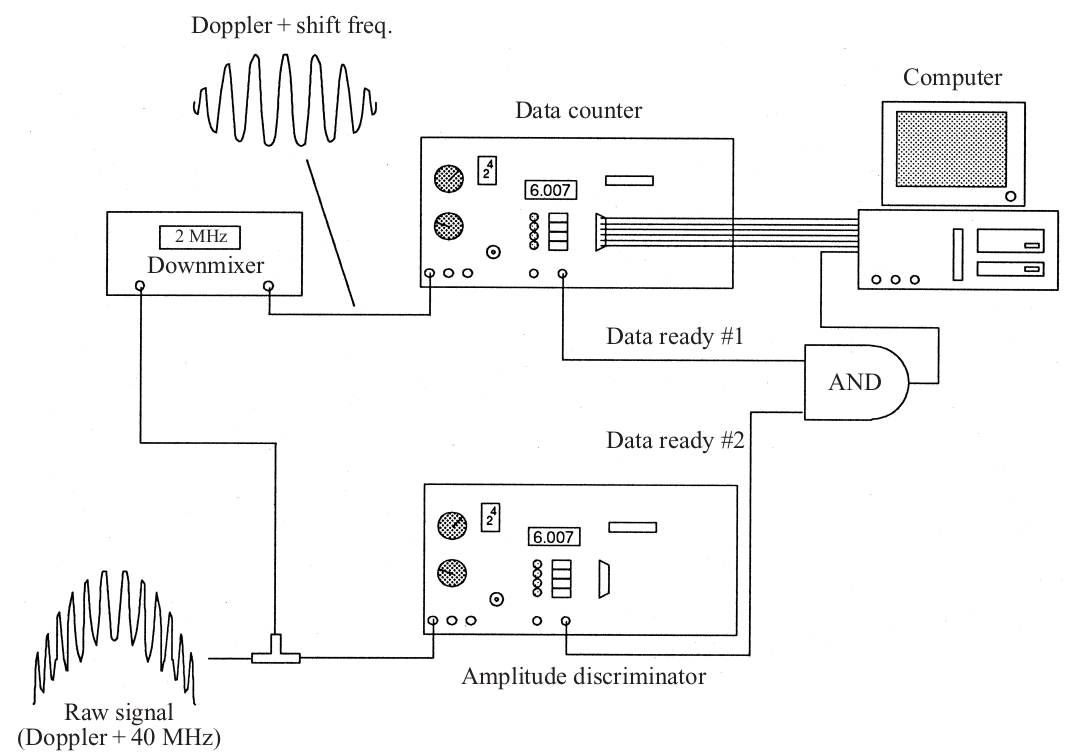
\includegraphics[width=0.68\textwidth]{Images/pedestal.png}
	\caption{Esquema del sistema de medici\'on de la interacci\'on part\'icula fluido$^{\cite{Fessler1999}}$.}
	\label{medicion}
\end{figure}

\noindent
\justify

El campo de densidad medio de part\'iculas se midi\'o al iluminar el material particulado a trav\'es de un pulso de frecuencia doble, $10 [mJ]$ por pulso de Neodimio, y al analizar diversas fotograf\'ias del experimento a trav\'es de un software de procesamiento de im\'agenes; permitiendo as\'i identificar cada part\'icula, su tama\~no y posici\'on en el lecho fluidizado.

\subsection{Resultados}

\noindent
\justify

Los perfiles de velocidad media se midieron, de manera experimental, a trav\'es de las condiciones especificadas en el Cuadro \ref{perfiles}. Pocas part\'iculas fueron identificadas en la zona de recirculaci\'on, por lo que no se reportaron datos en la zona $x/H = 2.5$ y $7$.

\begin{table}[h!]
	\centering
	\begin{adjustbox}{max width = \textwidth}
	\begin{tabular}{c c c c c}
		 & \multicolumn{2}{c}{\textbf{Direcci\'on de flujo}} & \multicolumn{2}{c}{\textbf{Direcci\'on normal al muro}} \\ \cmidrule{2-3}\cmidrule{4-5}
		 Clase de part\'icula & $x/H$ & Carga m\'asica & $x/H$ & Carga m\'asica \\ \hline
		 Vidrio de $90 [\mu m]$ & 2,5,7,9,14 & $20\%$ &  &  \\
		 Vidrio de $150 [\mu m]$ & 2,5,7,9,14 & $20\%, 40\%$ & 2,5,7,9,14 & $10\%$ \\
		 Cobre de $70 [\mu m]$ & -2, 0, 2, 5, 7, 9, 12 & $3\%, 10\%$ & 2,5,7,9,14 & $20\%$ \\
	\end{tabular}
	\end{adjustbox}
	\caption{Condiciones experimentales.}
	\label{perfiles}
\end{table}

\noindent
\justify

En la Figura \ref{resul1999} $a)$ se muestra el esquema de contorno de la densidad media de part\'iculas de cobre de $70 [\mu m]$. La velocidad m\'axima encontrada en este es, aproximadamente, de $0.2 U_0$. En la Figura \ref{resul1999} $b)$, se puede apreciar el esquema de contorno obtenido con base en el modelo CFD-DEM desarrollado.

\noindent
\justify

Cerca de la zona de salida del volumen de control, las velocidades de las part\'iculas exceden a las del gas debido a la desaceleraci\'on del fluido producida por la expansi\'on. La velocidad media de las part\'iculas en la direcci\'on del muro fue, generalmente, similar a las velocidades del fluido correspondiente.


\newpage

\begin{figure}[h!]
	\centering
	\begin{subfigure}[b]{\textwidth}
		\centering
		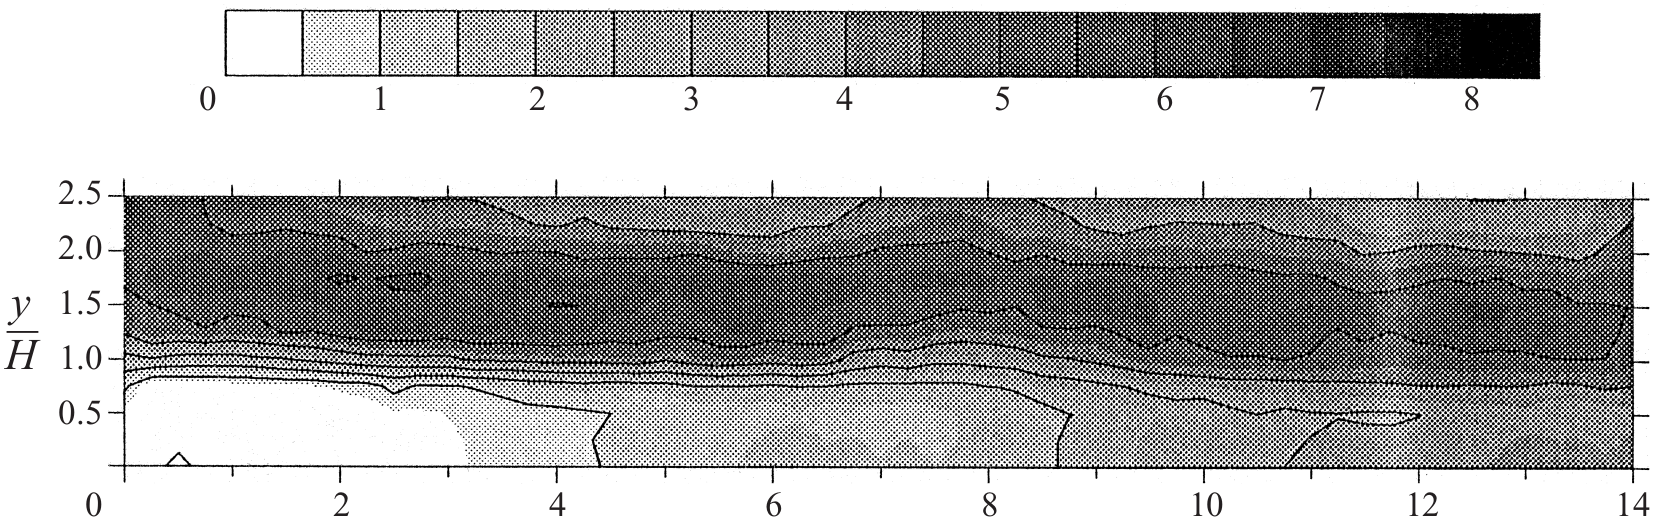
\includegraphics[width=\textwidth]{Images/contour1999.png}
		\caption{Diagrama de contorno de referencia de la densidad media de part\'iculas de cobre de $70 [\mu m]^{\cite{Fessler1999}}$.}
	\end{subfigure}
	\hfill
	\begin{subfigure}[b]{\textwidth}
		\centering
		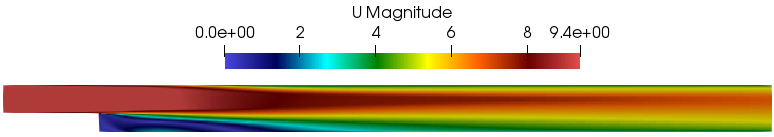
\includegraphics[width=\textwidth]{Images/valvel.png}
		\caption{Diagrama de contorno de la distribuci\'on de velocidad del sistema con part\'iculas de cobre de $70 [\mu m]$ - resultado obtenido al usar el modelo CFD-DEM desarrollado.}
	\end{subfigure}
	\caption{Comparaci\'on entre resultados del dise\~no experimental desarrollado por Fessler \& Eaton y los obtenidos a partir del modelo CFD-DEM desarrollado.}
	\label{resul1999}
\end{figure}

\noindent
\justify

Adicional al resultado mostrado en la Figura \ref{resul1999} $b)$, el modelo CFD-DEM desarrollado tambi\'en permite apreciar los resultados mostrados en la Figura \ref{valrel}.

\begin{figure}[h!]
	\centering
	\begin{subfigure}[b]{\textwidth}
		\centering
		
\includegraphics[width=\textwidth]{Images/valp.png}
		\caption{Diagrama de contorno de la distribuci\'on de la presi\'on dentro del volumen de control.}
	\end{subfigure}
	\hfill
	\begin{subfigure}[b]{\textwidth}
		\centering
		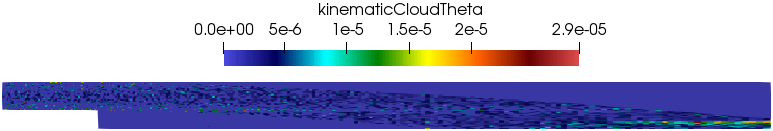
\includegraphics[width=\textwidth]{Images/valk.png}
		\caption{Diagrama de contorno de la variaci\'on de la fracci\'on de vac\'io en el volumen de control}
	\end{subfigure}
	\caption{Resultados obtenidos a partir del modelo CFD-DEM desarrollado.}
	\label{valrel}
\end{figure}

\noindent
\justify

La tendencia de distribuci\'on de las part\'iculas de cobre sobre el volumen de control se puede apreciar en la Figura \ref{valten}.

\begin{figure}[h!]
	\centering
	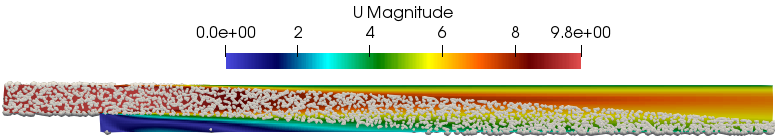
\includegraphics[width=1.1\textwidth]{Images/valpar.png}
	\caption{Distribuci\'on de las part\'iculas de cobre sobre la geometr\'ia.}
	\label{valten}
\end{figure}

\noindent
\justify

En la Figura \ref{valcompa} se puede apreciar la comparaci\'on directa en los perfiles de velocidad en diferentes puntos de inter\'es, contrastando los definidos por Fessler \& Eaton con respecto a los calculados por el modelo CFD-DEM desarrollado.

\begin{figure}[h!]
	\centering
	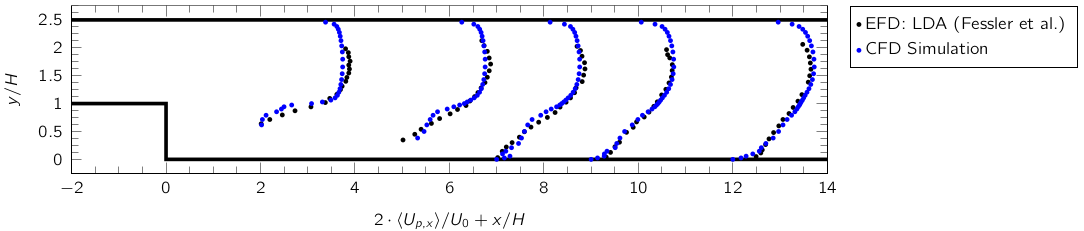
\includegraphics[width=1.1\textwidth]{Images/val.png}
	\caption{Comparaci\'on directa de los perfiles de velocidad experimentales con respecto al del modelo num\'erico desarrollado.}
	\label{valcompa}
\end{figure}

\noindent
\justify

En la Figura \ref{valcompa}, se puede apreciar una variaci\'on de hasta el $0.6\%$  entre los resultados experimentales con respecto a los obtenidos por el modelo num\'erico, reafirmando la exactitud de los resultados del modelo CFD-DEM; permitiendo as\'i validar el modelo desarrollado en el cap\'itulo \ref{CFD-DEM}.
